%%%%%%%%%%%%%%%%%%%%%%%%%%%%%%%%%%%%%%%%%
% Journal Article
% LaTeX Template
% Version 1.4 (15/5/16)
%
% This template has been downloaded from:
% http://www.LaTeXTemplates.com
%
% Original author:
% Frits Wenneker (http://www.howtotex.com) with extensive modifications by
% Vel (vel@LaTeXTemplates.com)
%
% License:
% CC BY-NC-SA 3.0 (http://creativecommons.org/licenses/by-nc-sa/3.0/)
%
%%%%%%%%%%%%%%%%%%%%%%%%%%%%%%%%%%%%%%%%%

%----------------------------------------------------------------------------------------
%	PACKAGES AND OTHER DOCUMENT CONFIGURATIONS
%----------------------------------------------------------------------------------------

\documentclass[twocolumn]{article}

\usepackage{blindtext} % Package to generate dummy text throughout this template 

\usepackage[sc]{mathpazo} % Use the Palatino font
\usepackage[T1]{fontenc} % Use 8-bit encoding that has 256 glyphs
\linespread{1.05} % Line spacing - Palatino needs more space between lines
\usepackage{microtype} % Slightly tweak font spacing for aesthetics


\usepackage[english]{babel} % Language hyphenation and typographical rules

\usepackage[hmarginratio=1:1,top=32mm,columnsep=20pt]{geometry} % Document margins
\usepackage[hang, small,labelfont=bf,up,textfont=it,up]{caption} % Custom captions under/above floats in tables or figures
\usepackage{booktabs} % Horizontal rules in tables

\usepackage{lettrine} % The lettrine is the first enlarged letter at the beginning of the text

\usepackage{enumitem} % Customized lists
\setlist[itemize]{noitemsep} % Make itemize lists more compact

\usepackage{abstract} % Allows abstract customization
\renewcommand{\abstractnamefont}{\normalfont\bfseries} % Set the "Abstract" text to bold
\renewcommand{\abstracttextfont}{\normalfont\small\itshape} % Set the abstract itself to small italic text

\usepackage{titlesec} % Allows customization of titles
\renewcommand\thesection{\Roman{section}} % Roman numerals for the sections
\renewcommand\thesubsection{\roman{subsection}} % roman numerals for subsections
\titleformat{\section}[block]{\large\scshape\centering}{\thesection.}{1em}{} % Change the look of the section titles
\titleformat{\subsection}[block]{\large}{\thesubsection.}{1em}{} % Change the look of the section titles

\usepackage{fancyhdr} % Headers and footers
\pagestyle{fancy} % All pages have headers and footers
\fancyhead{} % Blank out the default header
\fancyfoot{} % Blank out the default footer
\fancyhead[C]{Multi-Authority ABE for Bdrive$\bullet$ July 2018 $\bullet$ Vol. I, No. 1} % Custom header text
\fancyfoot[EL]{\thepage} % Custom footer text

\usepackage{titling} % Customizing the title section

\usepackage{hyperref} % For hyperlinks in the PDF
\usepackage{multicol}
\usepackage{graphicx}
\usepackage{caption}

  %
  \newcommand{\todo}[1]{
    \addcontentsline{tdo}{todo}{\protect{#1}}
    \marginpar{#1}
}

%----------------------------------------------------------------------------------------
%	TITLE SECTION
%----------------------------------------------------------------------------------------

\setlength{\droptitle}{-4\baselineskip} % Move the title up

\pretitle{\begin{center}\Huge\bfseries} % Article title formatting
\posttitle{\end{center}} % Article title closing formatting
\title{Multi-Authority Attribute Base Encyrption Scheme for Bdrive } % Article title
\author{%
\textsc{Marvin Petzolt}\thanks{TODO: fill} \\[1ex] % Your name
\normalsize TU Berlin \\ % Your institution
\normalsize \href{mailto:marvin.petzolt@protonmail.com}{marvin.petzolt@protonmail.com} % Your email address
%\and % Uncomment if 2 authors are required, duplicate these 4 lines if more
%\textsc{Jane Smith}\thanks{Corresponding author} \\[1ex] % Second author's name
%\normalsize University of Utah \\ % Second author's institution
%\normalsize \href{mailto:jane@smith.com}{jane@smith.com} % Second author's email address
}
\date{\today} % Leave empty to omit a date
\renewcommand{\maketitlehookd}{%
\begin{abstract}
\noindent TODO: Abstract % Dummy abstract text - replace \blindtext with your abstract text
\end{abstract}
}

%----------------------------------------------------------------------------------------

\begin{document}

% Print the title
\twocolumn[
    \maketitle
]


%----------------------------------------------------------------------------------------
%	ARTICLE CONTENTS
%----------------------------------------------------------------------------------------

\section{Introduction}

\lettrine[nindent=0em,lines=3]{B}
drive is a secure cloud storage where files get split up in smaller chunks that are saved speratly on different storage provider. To ensure end-to-end encryption a Bdrive client encrypts each of his chunks with the a one-time symmetric key that is then encrypted under his own public key. This encrypted key is called a file key and it is uploaded to the Bdrive server where it is stored securely. 

Since each device of the same user has a different private-public key pair, the client is in charge of making the file keys available for the new client. This is done by downloading each file key for the receptive file, downloading the public key of the new client, decrypting the file key with his own private key, encrypting it again with the public key of the new device and finally, uploading the new file key to the Bdrive server.

The number of file keys that need to be maintained raises with the number of clients. In addition Bdrive allows to share files between different users. The formula XXXX describes the number of file keys Bdrive need to store for each shared files between $u$ users, where each user $u_i$ has $d_i$ devices.

$$
n = \sum_{i \le u}{d_i} 
$$

Lets construct an example where the manager of a company wants to create a shared folder with all company employees. It is a medium sized company with 50 employees. At least haft of them have two Bdrive clients running. The manager wants to upload the 250 photos of the last company trip.
We end up by computing $3/2 * 50 * 250 = 18750$ file keys and for every new file uploaded 75 new file keys need to be uploaded. 

We reach the point where the classical public-key end-to-end encryption scheme does not scale anymore. 


\begin{figure*}[!ht]
\centering
    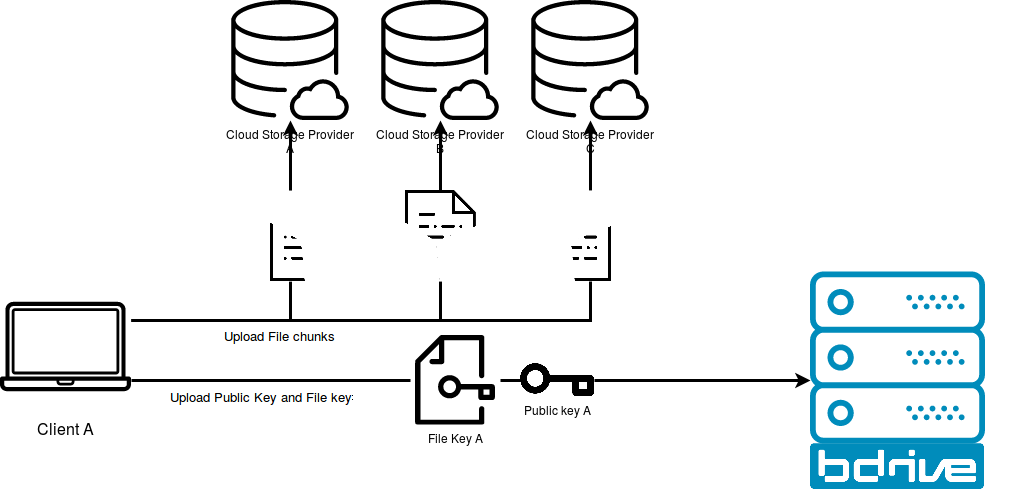
\includegraphics[width=0.7\linewidth]{img/bdrive1.png}\par 
    \caption{caption here}
\end{figure*}
\begin{figure*}[!ht]
\centering
    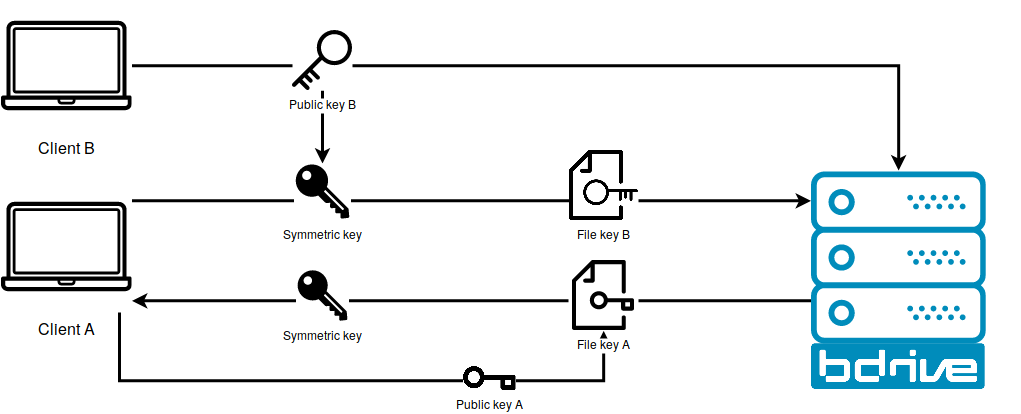
\includegraphics[width=0.7\linewidth]{img/bdrive2.png}\par
    \caption{caption here}
\end{figure*}


\section{Related Work}

Attribute Based Encryption (ABE), first introduced by Sahai and Waters \cite{sahai2005fuzzy}, is a cryptographic encryption scheme which encryptes under attributed that describe a user, rather than common known keys. This enables the encryptor to craft a cypher text over chosen attributes that can only be decrypted by any entity that holds a super set of matching attributes. Further, it is possible to embed the access policy in a tree inside the cipher text, where each node is contains \todo{fix encoding} “AND” or “OR” gates. If the attribute values are stored in the leafs, the decryptor can evaluate the tree in a post-order fashion and evaluate whether the root node yields “true” or “false”. This approach was first introduced by Bethencort, Sahai and Waters in Ciphertext-policy Attribute-Based Encryption (CP-ABE). \cite{bethencourt2007ciphertext}. 
It is also possible to do it the other way arround: Associate the user’s key with an access policy. Now, the encryptor needs only to encrypt the given plain text with the public key of specific attributes so that only user who hold the right keys are able to decrypt the cipher text. This approach is called Key-Policy Attribute Based Encryption (KP-ABE). \todo{cite} 
\todo{extend: Multi-ABE} 

%------------------------------------------------

\section{Security Requirements}
The core security requirements regarding Bdrive in the context of a multi-authority ABE scheme are the following:
\begin{itemize}
\item \textbf{Collusion resistance:} For two users it should not be possible to combine their attributes to archive a higher level 
\item \textbf{Inter-Company Sharing:} Since Bdrive would need to consider a multi-authority ABE scheme, it should not be possible for a company to decrypt or issue files of other companies if no explicit exception is given for certain files by a trusted company relationship. A companies attribute authority (AA) should be responsible for its domain. In the case of an inter company relationship, attributes needs to be issued across different companies. 
\item \textbf{Central Authority:} In a multi-authority setting usually a central authority is coordinating the different attribute authorities to identify users and prevent collusion. However, it should not be possible that the central authority has a global decryption power.  
\item \textbf{Secret Master key (if any):} Key recovery requires a secret and securely stored master key. It should solely function in the company domain and not globally. 
\item \textbf{Large Key Universe:} The key universe should be large so that Bdrive can act dynamically regarding attribution issuing and each company could define their own set of attributes. Further, a finite field of keys would restrict the number of possible users in the system, which is not intended.
\item \textbf{Adding new Attribute Authorities:} It should be possible to add new attribute authorities while runtime. Without either shutting down the system or recreating each key. 
\item \textbf{Key and Attribute revocation:} Either a period defining the lifetime of valid keys or a direct revocation mechanism ensures key and attribute revocation. In both cases the keys have a limited lifetime of two months. After this period the keys become invalid and have to be reissued.
Key attribute or whole key revocation should be possible to handle user management in terms of attribute promotion, attribute demotion and key revocation. Revoked keys are no longer able to decrypt the cypher text. 
\end{itemize}

On the other hand we are forced to loosen some security requirements that have hold in a RSA based environment. One Attribute Authority (AA) needs to issue the attributes for a group of users. This users are assigned to a designated company. Since the AA issues also the private keys for each attribute it holds also a master secret for this company domain and is in turn able to decrypt all users file of this company. While in the current cryptographic scheme enrolled in Bdrive an artificial master-key was implemented, it would still be possible to easily remove it from the system. This is not possible with the an ABE scheme. 


\section{Targets}
The target of this work will be to implement and define a multi-authority ABE scheme for Bdrive that fits the security requirements of the previous section. This approach will decrease the number of file keys stored on the Bdrive server dramatically and will make Bdrive scale better for a higher user workload. To evaluate this a prototype should be implemented that is able to up- and download files, to encrypt them symmetrically and encrypt the file key under a multi-authority ABE scheme. 

The minimal requirement is to implement a multi-authority ABE scheme where at least two AAs issue attributes to different users and the user are able to share a file between them. This file should only be encrypted using one file key. This implementation and system design summarized the security requirements of: Collusion resistance, inter-company Sharing, central authority, adding new authorities and Secret Master key. To implement and define this prototype Chase’s proposal of an multi-authority ABE scheme \cite{chase2007multi} in combination with the extension of Chase to deescalate the decryption power of the central authority \cite{chase2009improving} is used. 

The next step would be to implement the key-revocation, which is not trivial in an ABE setting. Optional is to extend the defined scheme with a large key universe. It is not clear yet whether this is even possible as it is proposed by Chase or if a complete different approach need to be taken to take this issue. 


%------------------------------------------------

\section{Concept}

%------------------------------------------------

\section{Method of Evalution}

%----------------------------------------------------------------------------------------
%	REFERENCE LIST
%----------------------------------------------------------------------------------------

\bibliography{multi-authority-abe-proposal} 
\bibliographystyle{ieeetr}

%----------------------------------------------------------------------------------------

\end{document}
